\documentclass[a4paper]{article}

\usepackage{mathtools}

\usepackage{amssymb}
\usepackage{geometry}
\usepackage{parskip}
\usepackage{tikz}
\usepackage{hyperref}
\usepackage{graphicx}

\usepackage{float}

\begin{document}
	
	\tableofcontents
	\newpage
\section{Overview}
Harder computational problems (Printer Scheduling, Sudoku, Coloring) can be solved by solving their logical encodings --- convert the problem to a logical formulation with boolean variables in disjunction (proposition) or variables in graphs (CSP).

Example problems solved by logical encodings
\begin{itemize}
	\item Syntax, checking for a well-formed program
	\item Type system, checking for a well-typed program
	\item Semantics, what happens when running a program
	\item Specification, check what the program is supposed to do
	\item Verification, prove that the program will never crash and meets spec
	\item Complexity, time/space complexity
\end{itemize}

Automata
\begin{itemize}
	\item Study of idealized computing machines
	\item How they work, can do
	\item Proving properties
\end{itemize}

Formal language theory
\begin{itemize}
	\item Study of sets of strings/words
	\item Related to automata theory
	\item Mapping grammars to automatas
\end{itemize}

Mathematic vocabulary
\begin{itemize}
	\item Natural language is ambiguous, must use maths/logic vocab
	\item Used in definition and proofs
\end{itemize}

Logic symbols
\begin{itemize}
	\item $\land$ AND, conjunction
	\item $\lor$ OR, disjunction
	\item $\implies$ Implies, implication
	\item $\lnot$ NOT, negation
\end{itemize}

A proposition/boolean encoding is to convert the program into a proposition statement of boolean variables.

\section{Formal Propositional Logic}
Propositional logic is equivalent to boolean logic with boolean variables. Boolean logic models logic algebraically similar to arithmetic.

Propositional formulas are built from
\begin{itemize}
	\item Atoms, $P, Q, R, P_1$ which are variables that are true or false
	\item Bottom, $\bot$ which is false
	\item Top, $\top$ which is true
	\item Negation, $\lnot P$
	\item Conjunction, $P \land Q$
	\item Disjunction, $P \lor Q$
	\item Implication, $P \rightarrow Q$ 
	\item With the bnf language syntax defined that a formula $\varphi$ being one of the above building blocks, with recursion in operands.
\end{itemize}

A (strict) well-formed-formula (wff) in logical proposition places explicit brackets around each infix/prefix operators, ignoring the convention of omitting parenthesis and operator precedence.

The IFF operand is defined by: $(P \leftrightarrow Q) \equiv (P \rightarrow Q) \land (Q \rightarrow P)$.

Conventions in writing propositional formula
\begin{itemize}
	\item Omit outer parenthesis unless precedence is wrong
	\item Negation has highest binding power (highest precedence). Implication has weakest binding power (lowest precedence).
	\item Precedence from weak to strong: implication, and/or, negation
	\item Imply is right associative, so $P \rightarrow Q \rightarrow R$ equivalent to $P \rightarrow (Q \rightarrow R)$
	\item AND/OR combined have ambigious precedence
\end{itemize}

Truth functions
\begin{itemize}
	\item A function from truth values to truth values 
	\item Truth values are boolean true and false
	\item Semantics of a truth function defined in a truth table using boolean variables
	\item A propositional formula is a truth function. We can view its subtree truth values under a truth table by writing columns of truth values under each atoms/operands.
\end{itemize}

Truth assignments
\begin{itemize}
	\item Propositional letters are boolean variables
	\item Truth assignment is a function from letters to truth values. In our case the assignments are explicit and complete
	\item Notation is
	\begin{align*}
		v &= \{P \rightarrow 1, Q \rightarrow 0\}\\
		v(P) &= 1\\
		v(Q) &= 0
	\end{align*}
	\item A formula will have a truth value under a truth assignment $v$.
	\item The shorthand $v \models P$ means $P$ is true under the truth assignment $v$. Equivalently, we say that $v$ is a model of (or models) $P$.
\end{itemize}

Logical equivalence
\begin{itemize}
	\item Formulas are equivalent iff they have identical truth values under every possible truth assignment. Equivalently if they have the same truth tables.
	\item Note that this means two formulas don't need the same variables to be equivalent if the assignment to that variable doesn't affect the equivalence.
	\item Shortand $P \equiv Q$ means that $P$ is logically equivalent to $Q$
\end{itemize}

Implication is weird since it doesn't mean causation. Stick to the logical definition that $$(P\rightarrow Q) \equiv (\lnot P \lor Q)$$

Modus Ponens
\begin{itemize}
	\item A argument to deduce a statement. The form of: $P \rightarrow Q$ (premise) is true, $P$ (premise) is true, so $Q$ (conclusion) is true
	\item A modus ponens argument is sound if: when conclusion $Q$ is true, the premise $P$ is also true (essentially the implication premise $P \rightarrow Q$ is true). Alternatively, when both the argument and premise are true the argument is sound.
\end{itemize}

Premise is a propositional statement that is true. Conclusion is a propositional statement that is inferred true from the premise using deductions.

\section{Semantic consequence}
Semantic consequence
\begin{itemize}
	\item For propositional statements $G$ and $F$, the statement $G$ is a semantic consequence of $F$ ($F \models G$) if and only if every model of $F$ is also a model of $G$.
	\item If $F \models G$, $F$ (semantically) entails $G$
	\item Can treat the ordering as implication ($F \models G, F \rightarrow G$)
	\item Used to relate two proposition statements where one is stronger than the other
\end{itemize}

Note that
\[
	A,B \models F
\]
is the same as
\[
	A \land B \models F
\]

Semantic consequence and equivalence
\[
	F \equiv G \iff F \models G \land G \models F
\]

Semantic consequence and implication
\begin{itemize}
	\item $$F \models G \iff \models F \rightarrow G$$, if $F$ entails $G$, then $F \rightarrow G$ is valid
	\item Importantly if the LHS of $\models$ is missing, any truth assignment is a model of the LHS, so the RHS is true under all models (valid)
	\item Collorary of
	\[
		F \equiv G \iff \models F \leftrightarrow G
	\]
\end{itemize}

\section{Satisfiability}
Terms
\begin{itemize}
	\item Tautology is a logical formula that is always true
	\item Contradiction is a logical formula that is always false. Negating a contradiction nets a tautology, vice versa.
	\item Valid statements are always true (tautology). Non-valid statements can sometimes be false. $\models F$ means $F$ is valid by definition
	\item Unsatistifiable statements are always false (contradiction). Satistifiable statements can sometimes be true.
	\item Contingent statements can sometimes be true, sometimes be false.
\end{itemize}

Substitution
\begin{itemize}
	\item The action of replacing all uses of a propositional variable (say $P$) with a given formula (say $Q\land R$)
	\item Substitution preserves the validity of the formula, and also preserves the unsatisfiability of it.
	\item Substitution does not preserve satisfiability, since we can replace the variable with a formula that is never true.
	\item Denote $F[A := B]$ as sub $A$ with $B$ in $F$.
\end{itemize}

Substitution preserves logical equivalence. Given $F,G,H$ formulas and any propositional variable $P$. If $F \equiv G$
\[
	F[P:=H] \equiv G[P:=H]
\]

Interchange of equivalence. If $F \equiv G$, we can replace $F$ with $G$ anywhere keeping all semantic properties. Formually, if $F \equiv G$
\[
	H[F := G] \equiv H
\]

Equivalence formats
\begin{itemize}
	\item Absorption
	\begin{align*}
		P \land P &\equiv P\\
		P \lor P &\equiv P
	\end{align*}
	\item Communtativity
	\begin{align*}
		P \land Q &\equiv Q \land P\\
		P \lor Q &\equiv Q \lor P\\
	\end{align*}
	\item Associativity of $\lor$ and $\land$
	\item Distributivity
	\begin{align*}
		P\land(Q\lor R) &\equiv (P\land Q) \lor (P\land R)
	\end{align*}
	\item $\leftrightarrow$ is commutative and associative
	\item Double negation
	\[
		P \equiv \lnot\lnot P
	\]
	\item De morgan
	\begin{align*}
		\lnot (P\land Q)\equiv \lnot P \lor \lnot Q
	\end{align*}
	\item Implication
	\[
		P \rightarrow Q \equiv \lnot P \lor Q
	\]
	\item Contraposition
	\begin{align*}
		\lnot P \rightarrow \lnot Q &\equiv Q \rightarrow P
	\end{align*}
	\item Biimplication
	\[
		P \leftrightarrow Q \equiv (P \land Q) \lor (\lnot P \land \lnot Q)
	\]
	\item Duality
	\begin{align*}
		\lnot \top \equiv \bot
	\end{align*}
	\item Negation from absurdity
	\[
		P \rightarrow \bot \equiv \lnot P
	\]
	\item Identity
	\[
		P \lor \bot \equiv P
	\]
	\item Dominance
	\[
		P \land \bot \equiv \bot
	\]
	\item Contradiction
	\[
		P \land \lnot P \equiv \bot
	\]
	\item Excluded middle
	\[
		P \lor \lnot P \equiv \top
	\]
\end{itemize}

\section{Resolution}
Propositional logic is decidable
\begin{itemize}
	\item it is always possible to check if a formula is valid/contingent/unsat using a truth table
	\item this takes finite $2^n$ checks with is slow
	\item there are more efficient methods of checking
\end{itemize}

Either-or reasoning
\begin{itemize}
	\item $(P \rightarrow F) \land (\lnot P \rightarrow G)\models F \lor G$ for any formula $F,G$ and proposition $P$
	\item This is a sound reasoning statement since the deduction obviously holds.
\end{itemize}

Resolution
\begin{itemize}
	\item Resolution is to apply either-or reasoning repeatly on a CNF to net several semantic consequences
	\item Resolution aims to solve the RHS of $A,B,C \models X$, finding the logical formula that is a semantic consequence of the premises
	\item For multiple premises, select (any) two that either-or reasoning can apply to and replace them to their semantic consequences.
	\item Can make a resolution graph by linking semantic consequences nodes to their premises
\end{itemize}

Refutation
\begin{itemize}
	\item If resolution shows that $A,B \models \bot$, the premises is a contradiction, and it is called a refutation
	\item This is because a semantic consequence of $\bot$ means no model sats premises
	\item To show that $F$ is valid, refute $\lnot F$ by showing $\lnot F \models \bot$
	\item To show that $F \models G$ (alt $F \rightarrow G$ is valid), refute $\lnot (\lnot F \lor G) \equiv F \land \lnot G \models \bot$
\end{itemize}

Failed refutation
\begin{itemize}
	\item If resolution cannot get a refutation and every possible semantic consequence is derived, the formula must be satisfiable
	\item The truth assignment that sats the formula can be read off by the single literal disjunction entailed in the resolution: the consequence of $P, \lnot Q$ means that $v = \{P \rightarrow \top, Q \rightarrow \bot\} \models F$  will sat the formula
\end{itemize}

Cancelling variables
\begin{itemize}
	\item Either-or reasoning will cancel/remove one variable if it is opposite in two premises
	\item Do not cancel multiple variables at once, like
	\[
		P\lor Q, \lnot P \lor \lnot Q
	\]
	this is not sound, as in that this argument is not correct
\end{itemize}

Formal resolution proof
\begin{itemize}
	\item A resolution proof of $C_m$ from wff $P_1, \dots, P_n$ is a string
	\[
		P_1,\dots,P_n \vdash C_1, \dots, C_m
	\]
	where either $C_i$ follows by resolution from any two wff earlier in the string
	\item It is essentially proving $C_m$ using a series of intermediate proofs involving $C_i$
\end{itemize}

Soundness
\begin{itemize}
	\item Writing $\Sigma \vdash F$ means that there is a resolution proof of $F$ from the premises $\Sigma$
	\item The $\vdash$ means deducing/follows
	\item The soundness theorem is that
	\[
		\Sigma \vdash F \implies \Sigma \models F
	\]
	from definition of resolution proofs using induction on $C_i$
\end{itemize}

\section{CNF}
An observation is that resolution is easier with premises in CNF.

Conjunctive Normal Form
\begin{itemize}
	\item Literal is a proposition atom (variable) or its negation
	\item Disjunctive clause is a disjunction of literals
	\item CNF is a conjunction of disjunctive clauses
	\item Examples
	\[
		(A\lor \lnot B) \land C
	\]
	\item Theorem, every formula has an equivalent CNF
\end{itemize}

Negation normal form
\begin{itemize}
	\item NNF means that connectives are $\land, \lor$ with negations only in front of variables
	\item We can get NNF from any formula:
	\item Eliminate $\leftrightarrow$ with $\land$ and $\rightarrow$
	\item Eliminate $\rightarrow$ with $\lor$ and $\lnot$
	\item Push $\lnot$ inwards using demorgan's law
	\item Eliminate $\lnot\lnot$
\end{itemize}

To convert from NNF to CNF, we only need to distribute $\lor$ over $\land$ using
\[
	A \lor (B \land C) \equiv( A\lor B) \land( A \lor C)
\]

Resolution is refutation-complete
\begin{itemize}
	\item We already know that resolution can deduce refutation implying unsatisfiability
	\item Theorem, every unsatisfiable formula can be refutated using resolution
	\item Formally, given clauses $\Sigma$, if $\Sigma \models \bot$ (it is unsat), then the $\Sigma \vdash \bot$ resolution proof must exist.
\end{itemize}

Satisfiability algorithm
\begin{itemize}
	\item Convert formula into CNF
	\item Apply resolution repeatly. If derives $\bot$, unsat. Otherwise when can't derive new formulas, sat
\end{itemize}

Simplifying CNF
\begin{itemize}
	\item Duplicated variables can be replaced with only one, $P\lor P \equiv P\land P \equiv P$
	\item Tautologies can be removed completely, $P \lor \lnot P \lor Q \equiv \top$
	\item Subsumptions can be removed. For formula $P$, if $(P\lor Q) \land P$, can remove $P$ to net $Q \land P$
	\item Note that CNF for a formula is not unique
\end{itemize}

Clausal form of CNF
\begin{itemize}
	\item Can write CNF as set of sets of literals: outer set for conjunction, inner set for disjunction
	\item For disjunction: $\{A,B\}$ represents $A \lor B$, $\{A\}$ represents $A$, $\{\}$ represents $\bot$ (since true iff at least one literal is true)
	\item For conjunction: $\{A,B\}$ represents $A \land B$, $\{A\}$ represents $A$, $\{\}$ represents $\top$ (sicne true iff all literals are true)
	\item Empty conjunction is valid, empty disjunction is unsat. Therefore, empty set of clauses is valid, set of empty clauses is unsat.
	\item To convert CNF to clausal form, replace $\lor$ in each conjunct with $\cup$, and literals $P$ with $\{P\}$
\end{itemize}

\section{Predicate Logic}
Propositional logic can encode some categories of problems where variables are either true/false, and our goal is to check whether a query is satisfiability (or valid).
\begin{itemize}
	\item However, some statements cannot be expressed adequately (nicely) in propositional logic. In particular when the problem contains:
	\item Infinite collections (every X)
	\item Transitive/relationship verbs (Loves)
	\item Relative pronouns (it, whoses)
\end{itemize}

Example predicate logic translations
\begin{itemize}
	\item No emus fly
	\[
		\forall x (Emu(x) \rightarrow \lnot Fly(x))
	\]
	\item There are black swans
	\[
		\exists x (Black(x) \land Swan(x))
	\]
	\item If all pushes the cart, then the donkey is happy
	\[
		(\forall x Push(x,c)) \rightarrow Happy(donkey)
	\]
	\item If anyone pushes the cart, the donkey is happy
	\[
		(\exists x Push(x, c)) \rightarrow Happy(donkey)
	\]
	\item Tina found Rover and returned him to Anne
	\[
		Found(tina, rover) \land Gave(tina, rover, anne)
	\]
	\item Tina found a dog and give it to Anne
	\[
		\exists x (Dog(x) \land Found(tina, x) \land Gave(tina, x, anne))
	\]
	\item Mother's mothers are grandmothers
	\[
		\forall x \forall y \forall z ((Mother(x, y) \land Mother(y, z)) \rightarrow Grandmother(x, z))
	\]
	\item No sorting algorithm can guarantee sorting with fewer than $n \log n$ comparisons
	\[
		\forall x (S(x) \rightarrow \lnot (c(x) < n\log n) )
	\]
\end{itemize}

Predicate logic new symbols
\begin{itemize}
	\item Constants. Often nouns represented as a lowercase letter. Begin of alphabet
	\item Predicates. Often verbs that take arguments with captialized names. Predicates with no arguments are propositional variables. Predicates must be truthy or falsy. Equality is a predicate with two arguments
	\item Quantifiers. $\forall$ forall and $\exists$ exists
	\item Variables. Lowercase letters used in quantifiers. End of alphabet. Its meaning can change compared to constants
	\item Functions. Lowecased names, taking constants as arguments. Forms a hierarchy on constants.
\end{itemize}

Existential quantification
\begin{itemize}
	\item Generalization of disjunction
	\item Example \[
		P(x_1) \lor P(x_2) \lor P(x_3) \leftrightarrow \exists x P(x)
	\]
\end{itemize}

Universal quantification
\begin{itemize}
	\item Generalization of conjunction
	\item Example \[
		P(x_1) \land P(x_2) \land P(x_3) \leftrightarrow \forall x P(x)
	\]
\end{itemize}

Quantifiers
\begin{itemize}
	\item The same quantifier is commutative.
	\item Different quantifiers are NOT commutative
\end{itemize}

Terms and atomic-formulas
\begin{itemize}
	\item Terms are individual objects that are not formulas. They can be: constants, variables, functions, numbers. Terms are not logical formulas and don't exist in propositional logic.
	\item Atomic formulas represents boolean statements on their argument objects. It is a single predicate applied to some terms. They are formulas
	\item Convention: terms/functions written with lowercase letters, atomic-formula/predicates written with uppercase letters
\end{itemize}

Predicate logic statement formal definition
\begin{itemize}
	\item Terms are built from variables, constants, and functions \[t ::= x | c | f(t,\dots) \]
	\item Formula are built from predicates, terms, connectives, and quantifiers
	\[
		\phi ::= P | P(t,\dots) | \bot | \top | (\lnot \phi) | (\phi \land \phi) | (\phi \lor \phi) | (\phi \rightarrow \phi) | (\forall x \phi) | (\exists x \phi)
	\]
	\item Note that $\forall, \exists$ have the same precedence as $\lnot$. Should omit parenthesis if we can
\end{itemize}

Predicates vs functions
\begin{itemize}
	\item Connectives: proposition inputs, proposition outputs
	\item Predicates: object inputs, proposition outputs
	\item Functions: object inputs, object outputs
\end{itemize}

Quantifier scope
\begin{itemize}
	\item The subformula attached to a quantifier is its scope
	\item The variable of the quantifier is bounded in the subformula (in its scope). A quantifier with variable $x$ binds $x$ within its scope.
	\item If a variable is not bounded, it is free
	\item Bound variables can be renamed unless there is a clash after it is renamed. Renaming free variables changing the meaning
\end{itemize}

Converting english to predicate logic
\begin{itemize}
	\item First identify nouns, verbs, pronouns, adjectives, relative clauses (parent of)
	\item Then assign: constants to singular nouns, predicates to verbs and adjectèves, functions to relative clauses, variables to indefinite pronouns
	\item Last, replicate logical structure of the sentence
	\item Be careful about the word ordering, they matter!
	\item Quantifiers are often implicit in english, look for (plural) nouns without determiners/constants (``Humans are mortal'' means ``All Humans'')
\end{itemize}

\section{Predicate Semantic Meaning}
Formula meaning
\begin{itemize}
	\item Meaning of a formula is about whether it is true or false
	\item Depends on the universal of objects (and interpretation) that we assign to the formula
	\item Predicate formulas can also be valid, contingent, or unsatisfiable (defined later)
\end{itemize}

Universe
\begin{itemize}
	\item A set of objects $U$ that we care about. Must be non-empty
	\item Quantifiers quantify over the universe
\end{itemize}

Interpretation function
\begin{itemize}
	\item Non-propositional-logic symbols are: predicates, function, and variables. They don't correspond to anything in the universe without an interpretation function
	\item Interpretation function maps every non-logical symbol to its (interpretation) object in the universe $U$:
	\item Constant mapped to an object $U$
	\item Predicate mapped to a relation on $U$, mapping objects (or tuple of objects) of $U$ to true or false
	\item Function mapped to a function from $U$ to $U$
\end{itemize}

Models
\begin{itemize}
	\item Model is a universe and interpretation function (that makes the formula true)
	\item A model for a formula implies that the formula is true under the model
	\item N with + is not a model for $\forall x \exists y (x+y = 1)$, since it is false under the model
\end{itemize}

Free variables
\begin{itemize}
	\item Free variables are variables that are not quantified over
	\item Variable assignment is a function $v$ that maps (free) variables to $U$.
	\item A formula with free variables may have its truthiness under model $M$ depend on the variable assignment
	\item Given an interpretation $I$, there is an automatic variable assignment function $v$ to even terms by natural extension
	\begin{align*}
		v(a) &= I(a)\\
		v(g(a,b)) &= I(g)(v(a), v(b)) = I(g)(I(a), I(b))
	\end{align*}
	Note that variables are excluded in this natural extension $v$
	\item Notation of $v_{x \to d}(y)$ means $v(y)$ except mapping $x$ to $d$
\end{itemize}

Formula truth
\begin{itemize}
	\item The truth of a closed formula depends only on the model. For a formula with free variables, it also depends on the variable assignment
	\item We are interested in variable assignments since it allows for a compositional approach to formula truth (recursive definition)
	\item In a model $M = (U, I)$ under variable assignment $v$:
	\item Atomic formula $P(t_1, \dots)$ is true iff $(v(t_1), \dots) \in I(P)$, essentially: convert predicate argument terms to objects, check if predicate with object is true under the interpretation
	\item Existential quantifier $\exists x F$ is true iff there is one $d \in U$ where $F$ is true in $M$ under $v_{x\to d}$
	\item Universal quantifier $\forall x F$ is true iff $\lnot \exists x (\lnot F)$ is true
	\item Connectives are true in the same way as under propositional logic
\end{itemize}

Quantifiers as two-player-games
\begin{itemize}
	\item If I make a claim that a formula is true, I get to choose the existential variables to make it true and the opposite gets to choose the universal variable to make it not true
	\item The selection order is done outside in
	\item Can use this to argument quantifier equivalences
\end{itemize}

Quantifier equivalences for general $F$ and $G$
\begin{align*}
	\forall x \forall y &\equiv \forall y \forall x\\
	\exists x \exists y &\equiv \exists y \exists x\\
	\lnot \forall x F &\equiv \exists x (\lnot F)\\
	\lnot \exists x F &\equiv \forall x (\lnot F)\\
	\exists x (F \lor G) &\equiv (\exists x F) \lor (\exists x G)\\
	\forall x (F \land G) &\equiv (\forall x F) \land (\forall x G)\\
	\exists x (F \to G) &\equiv (\forall x F) \to (\exists x G)
\end{align*}

Quantifier equivalences if $G$ has no free $x$ and for any $F$
\begin{align*}
	\exists x G &\equiv G\\
	\forall x G &\equiv G\\
	\exists x (F \land G) &\equiv (\exists x F) \land G\\
	\forall x (F \lor G) &\equiv (\forall x F) \lor G\\
	\forall x(F \to G) &\equiv (\exists x F) \to G\\
	\forall x (G \to F) &\equiv G \to (\forall x F)
\end{align*}

Semantic consequence
\begin{itemize}
	\item Write $M, v \models F$ to mean that $F$ is true under the model $M$ and variable assignment $v$. 
	\item Write $M \models F$ to mean that $M, v \models F$ under all variable assignments ($F$ is true in $M$, or $M$ is a model of $F$)
	\item Write $F \models G$, if every model of $F$ (models where $F$ is true) is a model of $G$ ($F$ semantically entails $G$).
	\item Write $F \equiv G$, if $F \models G, G \models F$ ($F$ equivalent to $G$)
\end{itemize}

Satisfiability
\begin{itemize}
	\item Consider a closed formula $F$
	\item $F$ is sat if $M \models F$ for some $M$
	\item $F$ is valid if $M \models F$ for all $M$
	\item $F$ is unsat if there are no $M$ where $M \models F$
	\item $F$ is non valid if there exists $M$ where $M \not \models F$
	\item $F$ is contingent if it is sat and not valid
	\item The same relationship between valid/unsat and non-valid/sat holds under $\lnot$.
\end{itemize}

\section{Resolution in Predicate Logic}
Extending resolution to predicate logic
\begin{itemize}
	\item Goal is to start with a predicate formula $F$, and then derive $\bot$
	\item CNF in predicate logic is a conjunction of disjunctions of literals, where all variables are assumed universally quantified
	\item Sadly, quantifiers means that not every predicate logic formula has a CNF. This means that we may give up equivalences when converting to CNF
\end{itemize}

Extended resolving to atomic formulas (variable, constants, functions)
\begin{itemize}
	\item Universally quantified either-or on predicates \[
		F(x) \lor G(x), \lnot G(a) \models F(a)
	\]
	\item Fixing variables in universial quantifiers, namely $G(x) \models G(a)$
	\[
		O(a, x), \lnot O(y, b) \models O(a,b), \lnot O(a,b), \bot
	\]
	Typically, we try to fix variables so that it matches constants in another similar disjunction
	\item In a resolution graph, write the variable assignment used when fixing variables for either-or reasoning
	\item When dropping forall, we can rename variables in different clauses.
	\item We can always duplicate a clause with another one with different variables
\end{itemize}

Eliminating existential quantifiers
\begin{itemize}
	\item If it is in front, like $F: \exists x \forall y P(x,y)$, we can derive that $G: \forall y P(a, y)$ for a constant $a$, then $G$ is satisfiable iff $F$ is satisfiable.  Note that this is not equivalence, and $a$ must be selected (or assumed selected) to maximize the possibility that $G$ sats.
	\item The $a$ is new and is called a skolem constant.
	\item If it is nested, like $F: \forall y \exists x P(x,y)$, there can be different $x$ for every $y$. We can derive that $G: \forall y P(f(y), y)$ is sat iff $F$ is sat. This assumes that $f(y)$ maps each $y$ to the value that may sat $G$.
	\item The function $f$ is new and is called a skolem function.
	\item If it is nested under multiple universal quantifier, make a skolem function taking multiple arguments
\end{itemize}

Predicate logic to clausal form (CNF)
\begin{itemize}
	\item Eliminate $\leftrightarrow$ and $\implies$
	\item Push negation in to NNF (treat universal as AND and existential as OR)
	\item Rename shadowed variables (no quantifier should use the same variable). Note that when forall a conjunctive clause, we can rename the forall variable within each conjunctive clauses
	\item Eliminate existential quantifier (skolemize)
	\item Drop universal quantifiers (directly drop them)
	\item Bring to CNF using distributive laws
\end{itemize}



\section{Formal Unification and Resolution}
Substitution
\begin{itemize}
	\item A function from variables to terms 
	\[
		\theta = \{x_1 \to t_1, x_2 \to t_2\}
	\]
	\item Given formula $E$, the substitution using $\theta$ will replace all occurances of $x_i$ with $t_i$, leading to
	\[
		E[\theta]
	\]
	\item Only do one pass of the subtitution, and not recurse using the newly substituted formula
\end{itemize}

Unifiers
\begin{itemize}
	\item A unifier of two expressions $s$ and $t$ is a substitution $\theta$ where
	\[
		s[\theta] = t[\theta]
	\]
	\item Two formulas $s$ and $t$ are unifiable iff there exists a unifier $\theta$ for $s$ and $t$.
\end{itemize}

Most general unifier (MGU)
\begin{itemize}
	\item A MGU for $s$ and $t$ is a substitution $\theta$ where: $\theta$ is a unifier for $s$ and $t$, every other unifier $\sigma$ can be expressed as $\tau \circ \theta$ for some substitution $\tau$ ($\forall \sigma, \exists \tau (\sigma = \tau \circ \theta))$
	\item Define the substitution composition $\tau \circ \theta$ as applying $\theta$ then $\tau$
	\item Essentially, MGU is the most general unifier that constrains as little variables as possible
	\item Theorem: If $s$ and $t$ are unifiable, there exists a MGU
	\item Note that terms must be finite: it cannot be a recursive definition or have infinite function  applications
\end{itemize}

Syntactic Unification Algorithm
\begin{itemize}
	\item Input: two expressions $s$ and $t$
	\item Output: the MGU if it is unifiable, failure if it is not
	\item Algorithm: \begin{enumerate}
		\item Start with the set containing $\{s=t\}$
		\item Perform one of the six actions, repeat
		\item Return result. If one assignment contains a variable assigned elsewhere, flatten/substitute the assignment for the final result.
	\end{enumerate}
	\item Actions:
	\begin{enumerate}
		\item For functions or predicates $F$ \[
			F(s_1, \dots) = F(t_1, \dots)
		\]
		replace it with $\{s_1 = t_1, \dots\}$
		\item For functions or predicates $F$ and $G$ \[
			F(s_1,\dots) = G(t_1, \dots)
		\]
		halt, failure
		\item $x=x$, delete the equation
		\item $t=x$, where $t$ is not a variable (t is a constant), replace it with $\{x=t\}$
		\item $x=t$, where $t$ is not $x$ but $x$ is in $t$, halt, failure
		\item $x=t$, where $t$ contains no $x$, save $\{x=t\}$ for solution, also substitute $x$ with $t$ everywhere else.
	\end{enumerate}
	\item To apply the algorithm, each step is a set of equality equations, with actions represented as arrows between two sets of equations.
	\item The algorithm always halts
	\item If it fails, no unifier exists
	\item If it unifiers, the resulting unifier is in normal form: every LHS is a different variable, no LHS appears in any RHS
	\item The resulting unifier is always a MGU
\end{itemize}

Resolution using Unification
\begin{itemize}
	\item Let $P_1$ and $P_2$ be unifiable atomic formulas with no common variables. Let $\theta$ be unifier
	\item Let $C_1$ and $C_2$ be disjunctive clauses, then \[
		C_1 \land P_1, C_2 \land \lnot P_2 \models (C_1 \lor C_2)[\theta]
		\]
	\item Basically, apply either-or using a MGU between the two complementory formulas
	\item The remaining resolution algorithm follows exactly like before
\end{itemize}

To prove that $A_1, \dots, A_n \models B$, we can refute
\[
	A_1 \land \dots A_n \land \lnot B
\]
using resolution.

Refutation proof shortcuts
\begin{itemize}
	\item To save space, can omit curly braces of clauses and omit parenthesis around function/predicate arguments
\end{itemize}


The unification algorithm is exponential on the length of the formulas. (For an example, consider the replacement of one term with a function with two identical terms).

To apply unification to type inference in a programming language, convert each function call expression with arguments $a$ and return value $b$ to
\[
f = a \to b = fun(a, b)
\]
and try to unify all such expressions to derive the MGU on all unknown types.

\section{Automatic Reasoning and Satisfiability}
Factoring
\begin{itemize}
	\item Consider clause $C$ with unifiable subformulas $A_1$ and $A_2$. Given mgu $\theta$, we can derive clause $C[\theta]$
	\item For example \[
		\{P(x), P(y)\} \equiv \{P(x)\}
	\]
	\item Sometimes needed to yield a refutation in resolution
\end{itemize}
 
Formal resolution method
\begin{itemize}
	\item Start with collection $\Sigma$ set of clauses
	\item While $\bot \not \in \Sigma$, do: add to $\Sigma$ a factor of some $C \in \Sigma$, or a resolvent between some $C_1,C_2\in \Sigma$.
	\item If MGU is used in resolution and factoring, the method is sound (correct) and refutation-complete (unsat formula iff resolution derives bottom in finite steps)
\end{itemize}

Resolution theorem
\begin{itemize}
	\item $\Sigma$ is unsat iff the resolution method can add $\bot$ after a finite number of steps
	\item Resolution process should be fair in unification by bfs instead of dfs
	\item Resolution is sound and refutation-complete
	\item It is not a decision procedure, as it may not terminate on finite formulas. No such procedures can ever exist for predicate logic.
	\item Validity and unsat are semi-decidable properties
\end{itemize}

Horn Clauses
\begin{itemize}
	\item A horn clause is a clause with at most positive literal. This means that each clause can be written as implication
	\item They are rules in prolog
	\item For propositional horn clauses, sat can be decided in linear time. This simplifies the search in logic programs
\end{itemize}

Horn clause sat algorithm
\begin{itemize}
	\item Maintain list containing $\bot$ and $\top$ in $\phi$
	\item Mark $\top$ if it is in list
	\item while there is a horn cluase $P_1 \land .. P_n \to Q$ in $\phi$ where all $P_i$ are marked and $Q$ is unmarked, mark $Q$
	\item If $\bot$ is marked, then unsat. Otherwise, return sat
	\item The sat assignment $v(P)$ is true if it is marked and false if it is not.
\end{itemize}

Equality in automated reasoning
\begin{itemize}
	\item Let $eq(X,Y)$ be a new predicate symbol
	\item Reflexivity, symmetry, transistivity, congurence
	\begin{align*}
		x &= x\\
		x=y &\iff y=x\\
		x=y\land y=z &\implies x=z\\
		x=y &\implies f(x) = f(y)\\
		x=y \land P(x) &\implies P(y)
	\end{align*}
	\item Using this axiomatic definition of equality tends to be quite inefficient
\end{itemize}

Automated reasoning
\begin{itemize}
	\item Main question, given a set of axioms $\{A_i\}$ and a conjecture $C$ in some formal language, do the axioms logically imply the conjecture?
	\item Example \[
	A_1, \dots, A_n \models C
	\]
\end{itemize}

Expressivity and automatizability
\begin{itemize}
	\item Expressivity is how nautrally computable problems are encoded
	\item Automatizability is finding a reasonably efficient sound and complete search
\end{itemize}

\section{Models of Computation}
Algorithm resources
\begin{itemize}
	\item Time
	\item Space
	\item Randomness
	\item Quantum entanglement
	\item Input access
\end{itemize}

Algorithms and computation problems
\begin{itemize}
	\item A computational problem is a specification: for every input $x$, what is the correct output. Represented as a predicate $P(x,y)$ which is true only when $y$ is the correct output for the input $x$
	\item An algorithm is an implementation (often for a computational problem): for every input $x$, what are the steps to obtain an (correct) output $y$. Represented as a function $A(x) = y$.
	\item Sorting is a computational problem. Quicksort is an algorithm for the sorting problem
	\item An algorithm $A(x)$ solves a problem $P(x,y)$ iff it sats the problem for all inputs 
	\[
		\forall x, P(x, A(x))
	\]
\end{itemize}

Algorithm efficiency
\begin{itemize}
	\item Can quantify the efficiency of an algorithm based on the resources it has access to.
	\item A computational model is the set of resource constraints
	\item Theoretical computer science concerns: power and limits of computational models, tradeoffs between resource usage between models
\end{itemize}

Simplified computational problems
\begin{itemize}
	\item Inputs are bitstrings (boolean strings)
	\item Outputs are YES/NO (single bit). This means a decision problem
	\item All problems can be reduced to solving this bitstring decision problem
	\item A computational problem modeled by a set of all bitstrings that are YES. Also known as a language $L$.
	\item The language of an algorithm (represented as $L(A)$) is the set of bitstrings that $A$ accepts. An algorithm $A$ recognizes a language $L'$ if $L(A) = L'$
\end{itemize}

\section{Finite (state) automata}
Key features
\begin{itemize}
	\item Memoryless, fixed memory for all input sizes
	\item Memorylessness, behavior depends only on the current state and next input. Does not remember information about past states
	\item Stream, does not know when the input ends
\end{itemize}

Definition
\begin{itemize}
	\item A finite state automata $M$ for an alphabet $\Sigma$ is a tuple $M = (Q, q_0, \delta, F, \Sigma)$
	\item $Q$ is the set of states
	\item $q_0 \in Q$ is the initial state
	\item $\delta : Q \times \Sigma \to Q$ is a transition function
	\item $F \subseteq Q$ is a set of accept states
	\item $\Sigma$ is a set of characters in the alphabet
\end{itemize}

State transition table
\begin{itemize}
	\item Describes $\delta$
	\item Each row describes: current state, transition if 0, transition if 1.
	\item To use the table, find row with current state, use transition rule depending on bitstring bit
\end{itemize}

State transition diagram
\begin{itemize}
	\item Visual description $\delta$
	\item Nodes are states, directed edges are transitions.
	\item Each edge labeled by 0 or 1 indicating the bit to cause this transition from the state.
	\item Double outlined states are accepted states
\end{itemize}

Bitstring decision algorithm
\begin{itemize}
	\item Denote a set of states $F$ as accept states.
	\item To run the automata on an input bitstring, repeatly apply $\delta$ on each bit of the input. If the final state is in $F$, the automata accepts the input. Otherwise, it rejects
	\item For example, given $x = v_0 v_1 \dots v_n$, the states are
	\begin{align*}
		r_0 &= q_0\\
		r_{i+1} &= \delta(r_{i}, v_i)
	\end{align*}
	\item Define $q(w)$ to be the automata state after processing the string $w$
	\item The sequence $r_0 \to r_1 \dots \to r_n$ is the computational path of $M$ on input $w$. It will be a path in the state transition diagram (allowing repeated vertices).
	\item The language $L$ recognized by an finite automata $M$ is just the set of bitstrings $x$ where $M(x)$. Or $L(M)$ where we treat $M$ as a decision algorithm.
\end{itemize}

Program analogy
\begin{itemize}
	\item Initialization, preinitialize set of variables (including isAccept), and transition function
	\item Input processing, while stream has characters, update variables using transition function
	\item When stream ends, return isAccept
\end{itemize}

\section{Regular Languages}
Regular language
\begin{itemize}
	\item A language $L$ is regular iff there exists a finite automaton that recognizes it (exists an $M$ such that $L(M) = L$)
\end{itemize}

Language universe
\begin{itemize}
	\item Given alphabet $\Sigma$, define $\Sigma^*$ to be the set of all strings built from the alphabet of any length, including the empty string $\epsilon$
	\item Any language $L$ over the alphabet $\Sigma$ is a subset of it $L \subseteq \Sigma^*$
\end{itemize}

String operations
\begin{itemize}
	\item The concatenation between strings $x$ and $y$ is denoted as $xy$
\end{itemize}

Language operations
\begin{itemize}
	\item Complement. $L^c$ is the set of strings $z$ in $\Sigma^*$ not in $L$
	\[
		L^c = \Sigma^* \setminus L
	\]
	\item Intersection. $A \cap B$ is the set of strings in both languages
	\[
		A \cap B = \{z \colon z \in A \land z \in B\}
	\]
	\item Union. $A \cup B$ is the set of strings in either language
	\[
		A \cup B = \{z \colon z \in A \lor z \in B\}
	\]
	\item Concatenation. $A\circ B$ is the set of strings $z$ such that it is a concat of strings from $A$ and $B$
	\[
		A \circ B = \{z \colon z = xy \land x \in A \land y \in B\}
	\].
	Define $L^k$ to be $L$ concat with itself $k$ times (or $\{\epsilon\}$ when $k=0$)
	\item Kleen star/closure. $L^*$ is the set of strings containing
	\begin{enumerate}
		\item the empty string $\epsilon$
		\item strings in $L^k$ for every positive $k$
	\end{enumerate} 
	\begin{align*}
		L^* &= \bigcup_{i=0}^{\infty} L^k \\
		&= \{\epsilon\} \circ L \circ L \dots \quad \text{assuming $L$ has the emptyset}
	\end{align*}
\end{itemize}

(Define) Regular operations are: union, concat, kleen star.

Concat rules
\begin{itemize}
	\item $L \circ \emptyset = \emptyset$
	\item $L \circ \{\epsilon\} = L$
	\item $A \subseteq A \circ B$ when $\epsilon \in B$
	\item Not commutative but is associative
\end{itemize}

Regular language closure
\begin{itemize}
	\item Regular languages are closed under all language operations
	\item $L$ regular implies that $L^*$ and $L^c$ are regular
	\item $A,B$ regular implies that $A\cup B$ and $A \cap B$ and $A \circ B$ are regular
	\item Note that this is implies not iff
	\item This means that given a finite automaton for $L$, we can get a finite automaton for $L^*$ and $L^c$. And if there is a finite automaton for $A$ and $B$, there is also one for $A \cup B$, $A \cap B$ and $A \circ B$
	\item Proof of closure takes the automaton for $L$, and derives a new automaton for $L$ under operation
\end{itemize}

\section{NFA}
Non-deterministic FA
\begin{itemize}
	\item The same as deterministic FA except \dots
	\item The transition function can return a subset of states $2^Q$, and it can also make transitions without consuming the next input character ($\epsilon$ transitions)
	\[
		\delta : Q \times (\Sigma \cup \{\epsilon\}) \to 2^Q
	\]
	\item On transition diagram: subset states means multiple possible transition path per state, $\epsilon$ transition means that there may be directed edges marked with $\epsilon$ that doesn't consume the input when transitioning
\end{itemize}

NFA acceptance (for NFA $N$)
\begin{itemize}
	\item A state $q$ is a resulting state after applying $w$ to $N$ iff there exists a sequence of state transitions where $q$ is the final state
	\item Denote $Q(w)$ as the set of all possible resulting states after applying input $w$ to $N$
	\item $N$ accepts a string $w$ iff $Q(w)$ contains an accept state.
	\item The language recognized by $N$ (denoted $L(N)$) is the set of strings that $N$ accepts 
\end{itemize}

Computation path (for NFA $N$)
\begin{itemize}
	\item A computation path is the sequence of states of $N$ while processing $w$
	\item The path is accepting if it ends in an accept state. The path is rejecting if it does not end in an accept state
	\item $N$ accepts $w$ iff there exists an accepting computation path
\end{itemize}

Theorems
\begin{itemize}
	\item Every DFA is a NFA, not the reverse
	\item Every NFA can be converted into an equivalent DFA
	\item Can prove the closure of regular languages by creating a NFA for the resulting language using the DFAs
\end{itemize}

\section{NFA Determination}
Machine equivalence
\begin{itemize}
	\item Two machines (like DFA/NFA) are equivalent if they recognizes the same language
\end{itemize}

NFA/DFA equivalence
\begin{itemize}
	\item Every NFA has an equivalent DFA
	\item Informally, this is derived from simulating the NFA. The steps are
	\begin{enumerate}
		\item Make the start state $q_0' = \{q_0, \dots\}$ including all states reached via $\epsilon$ transitions
		\item If $0$, find all the states reached from $q_0$ (or $\epsilon$ transition start states) using $0$ (or $\epsilon$ transitions). Call this $A$. Add transition from $q_0'$ to $A$. Similarly for $1$
		\item Repeat, for each state set $A$ and character $c$, add a transition to $B$ under $c$ where every character in $B$ can be reached by a state in $A$ following $c$ and $\epsilon$ transitions
		\item The starting state is $q_0'$. The accept states are all state sets $R$ such that it contains at least one accept state.
		\item State sets that are empty are dead states.
	\end{enumerate}
\end{itemize}

NFA to DFA algorithm
\begin{itemize}
	\item Let $N = (Q, \Sigma, \delta, q_0, F)$ be an NFA
	\item For all $R \subseteq Q$, define $E(R)$ be the $\epsilon$ closure of $R$. An element is in $E(R)$ if it is reached from a state in $R$ following 0 or more $\epsilon$ transitions
	\item Consider $M = (Q', \Sigma, \delta', q_0', F')$ be a DFA where:
	\item $Q' = P(Q)$
	\item $q_0' = E(\{q_0\})$
	\item $F' = \{R \in Q' | \exists c \in R, c \in F\}$
	\item $
	\delta'(R,a) =
		\bigcup_{r \in R} E(\delta(r,a))
	$
	\item Then the DFA $M$ is equivalent to NFA $N$
\end{itemize}

Closure proofs
\begin{itemize}
	\item Proof idea: Suppose that $A$ and $B$ are regular languages. There exists $N_1$ and $N_2$ DFA that recognizes them. Construct NFA $M$ that recognizes the combination of $A$ and $B$. Determinize $M$ into equivalent $N_3$ DFA. Then the combination is regular since $N_3$ recognizes it
	\item Formal proof. Define the two DFAs as tuples. Create NFA using functions of the two DFAs. Show that the NFA recognizes the new language
	\item Union, make $\epsilon$ transitions to start states of both DFA
	\item Concat, make $\epsilon$ transitions from accept states of $A$ to start state of $B$
	\item Kleen's star, create new initial accept state, add $\epsilon$ transition to start state. For every accept state, add $\epsilon$ transition to the old start state.
	\item Intersect
	\item Universal Complement
	\item Set subtract
	\item Reversal (reverse every accepted string)
\end{itemize}

\section{Minimization}
There may be multiple DFAs that recognizes the same language.

Minimal DFA
\begin{itemize}
	\item The minimal DFA for a regular language is a DFA that recognizes it with the minimum number of states
	\item The minimal DFA is unique. So we can check for DFA equivalence by computing the minimal DFA
\end{itemize}

Algorithms typically does not output a minimal DFA

Minimization
\begin{itemize}
	\item An algorithm that converts an NFA and produces the equivalent DFA
	\item First reverse the NFA
	\item Determinize the result
	\item Reverse again
	\item Determinize
\end{itemize}

Reversal
\begin{itemize}
	\item To reverse NFA $A$, assuming non-empty accept state
	\item If $F = \{q\}$, let $q$ be the accept state
	\item Otherwise, add new accept state $q$ with $\epsilon$ transitions from $F$ to $q$ (remove acceptance property of $F$)
	\item Reverse every transition in NFA. Let $q$ be start state and $q_0$ be the accept state.
\end{itemize}

\section{Regular Expressions}
Pattern matching
\begin{itemize}
	\item Search engines
	\item Lexical analysis
	\item Scripting language
	\item DNA
\end{itemize}

Regular expressions
\begin{itemize}
	\item Compact notation to describe regular languages
	\item Restricted syntax for pattern matching
	\item Used in most programming languages as regex
	\item Grammar over an alphabet $\Sigma$
	\begin{verbatim}
		regexp ::= a1 | ... | an | e | 0 | regexp U regexp | regexp o regexp | regexp* 
	\end{verbatim}
	\item Operator precedence: all concat omitt, star stronger than concat than union
\end{itemize}

Semantics (mapping regexp to formal languages)
\begin{itemize}
	\item $L(a) = \{a\}$
	\item $L(\epsilon) = \{\epsilon\}$
	\item $L(\emptyset) = \{\}$
	\item $L(R_1 \cup R_2) = L(R_1) \cup L(R_2)$
	\item $L(R_1 R_2) = L(R_1) \circ L(R_2)$
	\item $L(R*) = L(R)*$
\end{itemize}

Regular expression vs NFA
\begin{itemize}
	\item A language is regular iff it can be described by a regular expression (via semantics)
	\item Involves showing that regular expression only describes regular languages
	\item And that Regular languages must have a regular expression that describes it
\end{itemize}

Regular expression to regular language (NFA)
\begin{itemize}
	\item Inductive proof by building an NFA equivalent to the regular expression
	\item Base cases when $R = a, \epsilon, \emptyset$. Make these up
	\item Inductive cases when: $R = R_1 \cup R_2, R_1 \circ R_2, R_1^*$. Use the regular language closure under regular operations proof
\end{itemize}

Regular language to regular expression
\begin{itemize}
	\item Proof by converting an NFA to an equivalent regular expression
	\item Lemma: given an NFA, can build an equivalent NFA with at most one accept state
	\item Process:
	\begin{enumerate}
		\item Ensure that the NFA has one accept state (otherwise regexp is $\emptyset$)
		\item Convert all arcs to regexp
		\item Repeatly eliminate states that are neither start nor accept states. Create new arcs that are labeled by regexp
		\item At termination, there are two outcomes that can be directly translated to regexp
	\end{enumerate}
\end{itemize}

RL to Regexp state elimination
\begin{figure}[H]
	\centering
	\includegraphics[width=0.7\linewidth]{screenshot002}
	\caption{}
	\label{fig:screenshot002}
\end{figure}
Also note that we can replace multiple arcs between $A$ and $B$ by a single arc that unions all arcs.

RL to Regexp termination
\begin{figure}[H]
	\centering
	\includegraphics[width=0.7\linewidth]{screenshot001}
\end{figure}

Not much theory to say here, mostly just practice elimination and termination.

Regexp properties
\begin{itemize}
	\item $A \cup A = A$
	\item $A \cup B = B \cup A$
	\item $A \cup B \cup C = (A\cup B) \cup C$
	\item $A\circ B \circ C = (A \circ B) \circ C$
	\item $\emptyset \cup A = A$
	\item $\epsilon \circ A = A$
	\item $\emptyset \circ A = \emptyset$
	\item $(A \cup B) \circ C = (AB) \cup (AC)$
	\item $A \circ (B \cup C) = AB \cup AC$
	\item $(A^*)^* = A^*$
	\item $\emptyset^* = \epsilon^* = \epsilon$
	\item $(\epsilon\cup A)^* = A^*$
	\item $(A \cup B)^* = (A^* B^*)^*$
\end{itemize}

Limitations of finite automata
\begin{itemize}
	\item No lookahead
	\item Fixed number of bits of memory
\end{itemize}

\section{Proving Non-Regularity}
Two methods of non-regularity proving
\begin{itemize}
	\item Fooling sets (leveraging memoryless property)
	\item Closure properties (leveraging properties that some languages are not regular and that regular languages are closed)
	\item Pumping lemma (not covered coz it is too complicated)
\end{itemize}

Fooling set roadmap for language $L$
\begin{enumerate}
	\item Lower bound the number of states ($N$) for a DFA to have to recognize $L$. Stating: no DFA with fewer than $N$ states can recognize $L$
	\item Show that this lower bound $N$ exists for all natural numbers
	\item Hence the language is non-regular. (Since if it is, there exists DFA with $N$ states that recognize it, but the lower bound can be $N+1$, so this DFA doesn't recognize)
\end{enumerate}

Extended transition function
\begin{itemize}
	\item Define $\delta' : Q \times \Sigma^* \to Q$
	\[
		\delta'(q, w) = \begin{cases}
			q & \text{if}\quad w =  \epsilon\\
			\delta(r, a) & \text{if} \quad r = \delta'(q, x), w = xa, a \in \Sigma
		\end{cases}
	\]
	\item Essentially $\delta'(q, w)$ is the resulting automata state starting at $q$ following each character in string $w$.
	\item Theorem
	\[
		q(w) = \delta'(q_0, w)
	\]
	the resulting state of the automata when parsing $w$, $q(w)$, is equivalent to $\delta'(q_0, w)$.
\end{itemize}

Prefix-suffix decomposition
\begin{itemize}
	\item For string $w$, a valid prefix-suffix decomposition into strings $x, y$ means that $w = xy$. Note that both/either $x,y$ can be $\epsilon$
	\item For $w = xy$, we have
	\[
		q(w) = \delta'(q_0, w) = \delta'(q(x), y) = \delta'(\delta'(q_0, x), y)
	\]
\end{itemize}

Memoryless lemma
\begin{itemize}
	\item For strings $x,y$, if $q(x) = q(y)$, then for all strings $z$, $q(xz) = q(yz)$.
	\item Namely that future transitions/states depend only on: the current state $q(x)=q(y)$, and future inputs $z$
\end{itemize}

Characterizations of one-state dfas
\begin{itemize}
	\item One-state dfas can only recognize the languages: $\Sigma^*$ (accepts every string) or $\emptyset$ (rejects every string).
	\item Proof: every string has the same resulting state
\end{itemize}

Distinguishable pairs/suffix
\begin{itemize}
	\item Given language $L$, strings $x,y$ in general, $x$ and $y$ are distinguishable if there exists string $z$ such that only one of $xz$ and $yz$ is in $L$
	\item If $x,y$ are distinguishable, then the $z$ that distinguishes them is the distinguishing suffix
	\item Example: $L$ is set of all strings ending with $10$, then $0$ and $1$ are distinguishable with the distinguishable suffix $0$.
\end{itemize}

The memoryless lemma concerns only about finite state automata. Distinguishable pairs concern only about the underlying language. The combined lemma is
\begin{itemize}
	\item Given language $L$ and any DFA that recognizes $L$. For all distinguishable pairs $x,y$, 
	\[
		q(x) \neq q(y)
	\]
	\item Proof: distinguishable means that $q(xz) \neq q(yz)$, applying contrapositive memoryless lemma means that $q(x) \neq q(y)$
	\item Consequence: a language with at least one distinguishable pair is not recognized by any one-state DFA
\end{itemize}

Fooling set
\begin{itemize}
	\item A set of strings $F$ is a fooling set for language $L$ when every distinct pair in $F$ are distinguishable wrt $L$
	\item Fooling set lemma: if $F$ is a fooling set for language $L$, then every recognizing DFA for $L$ must have at least $|F|$ states
	\item Proof: suppose $M$ is a recognizing DFA with $k < |F|$ states, then notice that $q(x)$ is unique for all $x \in F$ by definition of the fooling set, with $|F|$ unique values. By the PHP, there must also be two strings in $F$ where $q(x) = q(y)$ ($|F|$ values out of $k<|F|$ states). Hence a contradiction.
\end{itemize}

Fooling set non-regularity theorem
\begin{itemize}
	\item If for every $k>0$, there exists a fooling set of size at least $k$, $|F| \geq k$, then the language cannot be regular
	\item Proof: Assume that the language is regular and there exists a DFA that recognizes it with $k$ states. Since there is a fooling set of size greater than $|F| \geq k + 1 > k$, the recognizing DFA must have at least $|F|$ states, which is impossible since it has only $k < |F|$ state. Hence a contradiction 
\end{itemize}

Fooling set examples
\begin{itemize}
	\item $L$ is set of strings ending with $10$, $F = \{\epsilon, 1, 10\}$
	\item $L$ is $\{0^n 1^n \colon n \geq 0\}$, $F_k = \{0^i \colon i \in [1..k] \}$
\end{itemize}

Fooling set construction strategies
\begin{itemize}
	\item Consider prefixes of strings in $L$
	\item Strings requiring a counter to differentiate between them, with the counter ranging from $1$ to $k$.
	\item Typically there is a unique distinguishable suffix that distinguishes one string in $F$ from all the others. (Not required in general since the suffix can change)
\end{itemize}

Minimal witness
\begin{itemize}
	\item A DFA is proved to be minimal for a regular language $L$ if there is a fooling set of size $|Q|$. If so, the fooling set $F$ is a witness to the minimal property of the DFA.
\end{itemize}

Closure non-regularity method
\begin{itemize}
	\item If $L^c$ is non-regular, then $L$ is non-regular
	\item If $A \cap B$ is non-regular, and $A$ is regular, then $B$ can't be regular
	\item Collorary: to prove that $L$ is non-regular, try proving that $L^c$ is non-regular; alternatively find a regular $B$ and prove $L \cap B$ is non-regular
\end{itemize}

Fooling set vs closure non-regularity
\begin{itemize}
	\item Fooling set will always work to prove non-regularity (theorem behind it)
	\item Closure methods are shorter and more concise, but may not always work and requires finding the right operations and languages.
\end{itemize}

\section{Context-free Language}
Context free grammar (CFG)
\begin{itemize}
	\item Defined as $G = (\Sigma, V, R, S)$
	\item $\Sigma$ is a finite set of terminal symbols
	\item $V$ is a finite set of variable symbols (nonterminals)
	\item $R$ is a finite set of production rules of the form $A \to w$, where $A$ is a variable and $w \in (\Sigma \cup V)^*$ is a string of variable/terminals. Also known as substitution rules. Allows recursion since $w$ can contain $A$.
	\item $S$ is the starting variable
\end{itemize}

CFG vs Regexp
\begin{itemize}
	\item Regexp allows us to create regular languages using regular operations
	\item CFG allows us to create context-free languages. Similar to regexp except that it can do recursion.
	\item Every language generated by Regexp can be generated by CFG, but not vice versa
	\item CFG used the define schemas of programming languages
\end{itemize}

CFG OR shorthand
\begin{itemize}
	\item Can combine production rules with the same LHS $A$ variable into a shorthand notation where each RHS is separated by \verb!|!
	\[
		A \to x | y | z
	\]
\end{itemize}

CFG string generation
\begin{itemize}
	\item Init output string $x = S$.
	\item While $x$ contains at least one variable, apply a production rule to replace a single occurrence of a variable in $x$.
	\item The final string with only terminals is the produced string
	\item Different rule selection leads to different final strings
\end{itemize}

Application and derivation
\begin{itemize}
	\item If applying $A \to y$ on string $xAz$ gives $xyz$, we say that $xAz \implies xyz$. This is application
	\item $x$ derives $z$ if there is a finite sequence of applications from $x$ to obtain $z$. We denote this as $x \implies^* z$.
	\item Formally, $x \implies^* z$ when: $x=z$, or there exists strings $y_1, \dots y_n$ where
	\[
		x \implies y_1 \implies \dots y_n \implies z
	\]
	\item The sequence to derive $z$ is called the derivation of $z$.
\end{itemize}

Sentential
\begin{itemize}
	\item Strings in $(\Sigma \cup V)^*$ are in sentential forms
	\item Strings in $\Sigma^*$ are sentences
	\item Sentences are sentenetial form without variables
\end{itemize}


CFG language
\begin{itemize}
	\item The language generated by a CFG is the set of strings that the CFG can generate.
	\item Equivalently, this is the set of strings that can be derived from the start variable
	\[
		L(G) = \{ x \colon S \implies^* x\}
	\]
\end{itemize}

Context free language
\begin{itemize}
	\item A language is context free iff there exists a CFG that generates it
\end{itemize}

Parse tree
\begin{itemize}
	\item A visualization of the derivation process from $S$.
	\item Represents the syntactic structure of a string. Namely, the tree should tell us the order of operations to compute if the language is arithmetic expression.
	\item Formally, a parse tree for a string $w \in L(G)$ is a root tree
	\begin{itemize}
		\item Each node is labeled by a variable or a terminal
		\item Root node is $S$
		\item Non-leaf nodes are associated with a production rule $A\to v$. Namely, $A$ is the non-leaf node label and each symbol in $v$ are its child node labels from left-to-right
		\item Leaf nodes are all terminal. The concat of all leaf nodes from left-to-right gives $w$
	\end{itemize}
\end{itemize}

Ambiguity
\begin{itemize}
	\item A string is ambiguous against a grammar $G$ iff there are more than one parse tree for the string.
	\item A grammar $G$ is ambiguous iff there exists an ambiguous string with respect to it 
	\item A context-free language $L$ is inherently ambiguous iff every $G$ that generates it are ambiguous
\end{itemize}

Closure
\begin{itemize}
	\item The class of context-free languages are closed under: union, concat,  kleene's star, reversal
	\item It is NOT closed under intersection. However, $A \cap R$ is context free if $A$ is context free and $R$ is regular 
	\item To prove closure, take the two grammars and make a new context-free grammar that generates the new language
\end{itemize}

Closure proofs
\begin{itemize}
	\item Union: Make a new start variable with production rule \verb!S1 -> Sa | Sb! pointing to the start variable on $A$ and $B$
	\item Kleene's star: make a new start variable with production rule \verb!S1 -> e | Sa S1!
	\item Concat: new start variable with rule that is concat start variables
	\item Reversal: reverse all strings in rules
\end{itemize}

Regular languages
\begin{itemize}
	\item Every regular language is context free
	\item Proof: $A$ is a regular language, $R$ is a regular expression that matches it, recursively convert the regexp to CFG rules and variables using the regexp operations (union, concat, kleenestar, atom)
	\item To convert regexp to CFG: convert each regexp operation to production rule inside out
\end{itemize}

Example conversion $(0 \cup 1)^*$
\begin{verbatim}
S -> A
A -> e | BA
B -> C | D
C -> 0
D -> 1
\end{verbatim}

\section{Push-down automata}
Machines and Languages
\begin{itemize}
	\item Finite Automata and Regular languages
	\item Pushdown automata and Context-Free languages
	\item Linear-bounded automata and Context-Sensitive
	\item Halting-turning machine and decidable
	\item Turing machine and turing recognizable
\end{itemize}

Pushdown automata
\begin{itemize}
	\item An NFA with an unlimited stack memory
	\item Stack operations: peak stack, push stack, pop stack
	\item A pushdown automata is defined by the tuple $P = (Q, \Sigma, \Gamma, \delta, q_0, F)$ where 
	\item $Q$ is the set of states
	\item $\Sigma$ is the alphabet set of the input string
	\item $\Gamma$ is the alphabet set of the stack
	\item $\delta : (Q \times \Sigma_\epsilon \times \Gamma_\epsilon) \to \mathcal{P}(Q \times \Gamma_\epsilon)$, a function mapping (current state, input symbol, stack symbol) to a set of (next state, new stack symbol)
	\item $q_0 \in Q$ is the starting state
	\item $F \subseteq Q$ is the set of accepting states
\end{itemize}

PDA operations
\begin{itemize}
	\item TLDR, The PDA accepts if there exists a path (non-deterministically) that ends in an accept state. Similar to NFA except with stack operations
	\item Starts at $q_0$
	\item Repeat while still input: non-deterministically transition via a valid transition from $\delta$ to a new state \verb|a, b -> c|, consume input $a$, replace stack top $b$ with $c$. Reject if no transitions are possible
	\item Accept if state in accept state.
\end{itemize}

Pushdown automata transitions
\begin{itemize}
	\item Of the form: $A, B \to C$ where
	\item $A$ is the input character
	\item $B$ is the stack top character that is popped ($\epsilon$ implies no pop and matches any stack symbol)
	\item $C$ is the character to be pushed onto the stack ($\epsilon$ implies no push)
	\item Example: \verb|_, e -> e| means noop,\\ \verb|_, a -> e| means popping \verb|a|,\\ \verb|_, e -> a| means pushing \verb|a|,\\ \verb|_, a -> b| means swapping \verb|a| with \verb|b|
\end{itemize}

Pushdown automata empty stack
\begin{itemize}
	\item No requirement for the stack to be empty to be accepted
	\item To ensure an empty stack, can push a special character \verb|$| onto the stack at the start, and pop it at the end transitioning to an accept state.
	\item If the stack is empty, a pop operation that is not $\epsilon$ is invalid. Any PDA that may perform this operation is invalid
\end{itemize}

The PDA to recognize $\{w w^R \colon w \in \{0,1\}^*\}$

\begin{figure}[h]
	\begin{center}
		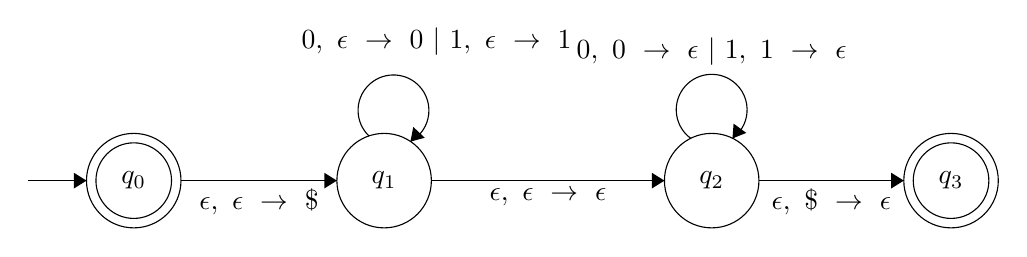
\begin{tikzpicture}[scale=0.2]
			\tikzstyle{every node}+=[inner sep=0pt]
			\draw [black] (14.7,-31.7) circle (3);
			\draw (14.7,-31.7) node {$q_0$};
			\draw [black] (14.7,-31.7) circle (2.4);
			\draw [black] (30.6,-31.7) circle (3);
			\draw (30.6,-31.7) node {$q_1$};
			\draw [black] (51.4,-31.7) circle (3);
			\draw (51.4,-31.7) node {$q_2$};
			\draw [black] (66.6,-31.7) circle (3);
			\draw (66.6,-31.7) node {$q_3$};
			\draw [black] (66.6,-31.7) circle (2.4);
			\draw [black] (17.7,-31.7) -- (27.6,-31.7);
			\fill [black] (27.6,-31.7) -- (26.8,-31.2) -- (26.8,-32.2);
			\draw (22.65,-32.2) node [below] {$\epsilon,\mbox{ }\epsilon\mbox{ }\to\mbox{ }\$$};
			\draw [black] (29.643,-28.869) arc (226.40536:-61.59464:2.25);
			\draw (33.93,-23.78) node [above] {$0,\mbox{ }\epsilon\mbox{ }\to\mbox{ }0\mbox{ }|\mbox{ }1,\mbox{ }\epsilon\mbox{ }\to\mbox{ }1$};
			\fill [black] (32.27,-29.22) -- (33.18,-28.98) -- (32.45,-28.29);
			\draw [black] (33.6,-31.7) -- (48.4,-31.7);
			\fill [black] (48.4,-31.7) -- (47.6,-31.2) -- (47.6,-32.2);
			\draw (41,-32.2) node [below] {$\epsilon,\mbox{ }\epsilon\mbox{ }\to\mbox{ }\epsilon$};
			\draw [black] (50.077,-29.02) arc (234:-54:2.25);
			\draw (51.4,-24.45) node [above] {$0,\mbox{ }0\mbox{ }\to\mbox{ }\epsilon\mbox{ }|\mbox{ }1,\mbox{ }1\mbox{ }\to\mbox{ }\epsilon$};
			\fill [black] (52.72,-29.02) -- (53.6,-28.67) -- (52.79,-28.08);
			\draw [black] (54.4,-31.7) -- (63.6,-31.7);
			\fill [black] (63.6,-31.7) -- (62.8,-31.2) -- (62.8,-32.2);
			\draw (59,-32.2) node [below] {$\epsilon,\mbox{ }\$\mbox{ }\to\mbox{ }\epsilon$};
			\draw [black] (8,-31.7) -- (11.7,-31.7);
			\fill [black] (11.7,-31.7) -- (10.9,-31.2) -- (10.9,-32.2);
		\end{tikzpicture}
	\end{center}
	\caption{PDA to recognize panlindromes}
\end{figure}

Context-free language
\begin{itemize}
	\item A language is context-free iff there exists a PDA that recognizes it
	\item PDA has equivalent power as CFG
\end{itemize}

Regular grammars
\begin{itemize}
	\item Regular grammars (grammar that generates regular languages) are CFG with restricted rules
	\item The restrictions are: they must be of form $A \to w$ or $A \to w B$, where $A, B \in V$ and $w \in \Sigma^*$
\end{itemize}

\section{PDA and CFG}
CFG = PDA
\begin{itemize}
	\item A language can be generated by a CFG iff it is recognized by a PDA
	\item Proof requires proving both ways: every CFG has a PDA, every PDA has a CFG
\end{itemize}

If language can be generated by CFG, there exists a PDA that recognizes it
\begin{itemize}
	\item Given CFG $G$, consider a PDA with alphabet of the terminals and variables of $G$
	\item PDA start by pushing start variable onto stack (assuming empty stack symbol first)
	\item If top of stack is a variable, non-deterministically choose a production of the variable from $G$. Pop variable from stack and push the RHS of the rule onto stack in reverse order
	\item If top symbol is a terminal, pop it from stack if it matches current input symbol. Otherwise reject
	\item When stack is empty, accept if the input is empty, reject otherwise (link all states to a stackempty state with $\epsilon$ transition and empty stack symbol)
\end{itemize}

The reverse direction (PDA to CFG)
\begin{itemize}
	\item Simplify the PDA to follow the conditions: single accept state, empty stack when accept, transitions only pushes char to stack or pops char from stack.
	\item Then we can directly create the CFG from PDA using \url{https://www3.nd.edu/%7Edchiang/teaching/theory/2016/notes/week06/week06b.pdf}
	\item The idea is to create variables $A_{pq}$ that generates strings which corresponds to strings accepted from state $p$ to $q$
\end{itemize}

Note that non-deterministic pushdown automata are strictly more powerful than deterministic versions, unlike DFA.

Can use pumping lemma to prove a language is not context-free, not examinable.

\section{Turing Machine}
Informal Turing Machine
\begin{itemize}
	\item Consists of an input tape and a finite state machine
	\item The head can read and write on the input tape
	\item The head can move left or right
	\item The input tape is infinite to the right
	\item Infinitely many blank characters following the input on the tape
	\item The machine can accept or reject the input at any time (not just the input end)
\end{itemize}

Example TM for $\{ a^n b^n c^n \colon n \geq 0\}$
\begin{itemize}
	\item Scan right until blank while checking if input is in $a^* b^* c^*$. Reject if not
	\item Return head to left end
	\item Scan right, crossing off a single a, b, and c (by replacing them with the crossed character)
	\item If last one of each symbol, accept (make matching states indicating seeing uncrossed input)
	\item If last one of one symbol but not others, reject
	\item Otherwise, return to left end and repeat
\end{itemize}

Turing Machine
\begin{itemize}
	\item $TM = (Q, \Sigma, \Gamma, q_0, q_a, q_r, \delta)$
	\item $\Sigma$ is the input alphabet
	\item $\Gamma$ is the tape alphabet ($\Sigma \subseteq \Gamma$) that has a blank character
	\item $q_0$ is initial state
	\item $q_a, q_r$ are accept and reject states
	\item $\delta : Q \times \Gamma \to Q \times \Gamma \times \{L, R\}$
	\item The transitions $\delta(q, a) = (p, b, L)$ implies that from state $q$ with tape input $a$, transition to state $p$, writing $b$ to tape, move left
	\item Note that this TM is deterministic. $\delta$ also needs to be complete (requiring all transitions) for all states except for $q_a, q_r$
	\item Moving left when the tape head is on the left-most tape character does nothing
\end{itemize}

Termination
\begin{itemize}
	\item On an input $w$ the TM may halt (reached $q_a, q_r$) or loop forever
	\item There are three possible outcomes for each $w$: accept $w$ by entering $q_a$ (halt), reject $w$ by entering $q_r$ (halt), loop
\end{itemize}

TM language
\begin{itemize}
	\item $L(M)$ is defined as the set of strings that can be accepted by $w$.
	\item Strings that are rejected or loop forever without accepting are not in $L(M)$
\end{itemize}

Decider
\begin{itemize}
	\item A TM is a decider if it halts on all inputs. It will never loop
\end{itemize}

TM graph
\begin{itemize}
	\item States are nodes
	\item Transitions: \verb|a -> b, R| means tape input $a$ overwriting with $b$ and move right; \verb|a -> L| means tape input $a$ not overwriting, move left
	\item An DFA can be converted to TM by replacing $a$ with \verb|a -> R|
\end{itemize}

TM configurations
\begin{itemize}
	\item A configuration for TM is a snapshot of its execution containing: current sate, current tape values, current location of head on tape
	\item A configuration is represented by \verb|abqabb| where $q$ is the state on the left of the tape head location.
	\item The initial configuration for input $w$ is always $q_0w$
	\item If applying $\delta$ on config $C$ yields $C'$, then $C \Rightarrow C'$. For instance
	\begin{align*}
		uqbv \Rightarrow uctv &\quad \delta(q, b) = (t, c, R)\\
		qbuv \Rightarrow tcuv &\quad \delta(q, b) = (t, c, L)
	\end{align*}
	\item TM accepts a string $w$ iif there exists a sequence $C_1, C_2, \dots, C_k$ where: $C_1 = q_0 w$, and $C_i \Rightarrow C_{i+1}$, and state of $C_k$ is $q_a$.
\end{itemize}

Recognizer and Deciders
\begin{itemize}
	\item $M$ recognizes a language $A$ iff $A = L(M)$. And $A$ is turing-recognizable iff there exists a TM that recognizes it
	\item $M$ decides a language $A$ iff $A = L(M)$ ($M$ recognizes $A$) and that $M$ is a decider ($M$ always halts). And $A$ is turing-decidable iff there exists a TM decider that recognizes the langauge
	\item All turing-decidable languages are turing-recognizable, since there exists a TM that recognizes it.
\end{itemize}

Satisifiability
\begin{itemize}
	\item Satisifiability in propositional logic is decidable
	\item Satisifiability in first-order logic is only recognizable
\end{itemize}

\section{Church Turing Thesis}
Church Turing Thesis
\begin{itemize}
	\item All reasonable models of unrestricted computation (lambda calculus, random access machine, programming language) are equivalent to the power of the turing machine
	\item Prefer turing machine since it is simple and familiar
	\item Essentially: all problems that are computable under any computer (solvable) must also be decidable, and vice versa. This holds even with quantum computers, time travelling, and non-determinism.
\end{itemize}

Turning machine is robust
\begin{itemize}
	\item Adding new features to it doesn't make it more powerful
\end{itemize}

Multi-tape turing machines
\begin{itemize}
	\item Multiple set of tapes (input tape, multiple work tapes initially blank). Number of work tapes fixed at the start
	\item Transition depends on all head symbols on all tapes. Can modify each tape individually on a transition
\end{itemize}

Multi-tape theorem
\begin{itemize}
	\item Language $A$ is t-recognizable iff there exists a multi-tape turing machine that recognizes it
	\item Forward direction proof obvious
	\item To convert a multi-tape TM into a single tape $S$:
	\begin{itemize}
		\item $S$ stores multiple tapes on a single tape in blocks separated by character \verb|#|
		\item Make a dotted variant for tape symbols to indicate tape head in eaceh block
		\item To simulate a transition: scan entire tape to find dotted symbols, scan again to update $S$ according to multi-tape $\delta$
		\item If ran out of space in a block, shift everything after updating (leave an empty space after each block)
		\item The set of states (including $q_a, q_r$) are equivalent to multi-tape. So same accept/reject criteria
	\end{itemize}
\end{itemize}

Non-deterministic turing machine
\begin{itemize}
	\item A NTM is similar to a DTM except that its $\delta$ maps to $\mathcal{P}(Q \times \Gamma \times \{L,R\})$
\end{itemize}

NTM theorem
\begin{itemize}
	\item Language $A$ is t-recognizable iff there is a NTM that recognizes it
	\item Forward direction is obvious
	\item To convert a NTM into DTM:
	\begin{itemize}
		\item See that a NTM creates a computation tree with threads of non-deterministic operations
		\item The tape will store blocks of tape each corresponding to a computation fork/thread of the NTM.
		\item Head of each block stored using dotted variant
		\item State of each block stored as a symbol at the start of each block
		\item Copy block state if fork
		\item Accept if any block state is $q_a$, reject if any block state is $q_r$
	\end{itemize}
\end{itemize}

\section{TM Algorithms on Automatas}
String encodings for TM
\begin{itemize}
	\item For any object $O$, denote $\langle O \rangle$ as the string encoding of that object.
	\item Every discrete object has an string representation
	\item For a list of objects $O_1, \dots, O_n$, write $\langle O_1, \dots, O_n \rangle$ to be the encoding of all objects into a single string (encode each separated by a separator character)
\end{itemize}

Turing machine notation
\begin{itemize}
	\item To describe TM algorithms, use high level english descriptions
	\item In principle we can convert the descriptions into states/transition-functions
	\item Notation to writing TM $M$ is: $M$ = ``On input $w$, blah english description of algorithm''
\end{itemize}

Automata problems
\begin{itemize}
	\item Acceptance problem involves a TM checking if an automata accepts an input
	\item Emptiness problem involves a TM checking if an automata recognizes the $\emptyset$ language (no string is accepted). This is similar to checking unsat
	\item Equivalence problem involves a TM checking if two automatas are equivalent
\end{itemize}

DFA acceptance problem
\begin{itemize}
	\item Let $A_{DFA} = \{\langle B, w \rangle \colon \text{B is DFA, B accepts w}\}$
	\item Theorem is that $A_{DFA}$ is decidable. That is, there exists a turing machine (which always halts) that can recognize the language
	\item The TM $D_{A-DFA}$ that decides it is
	\begin{itemize}
		\item On input $s$
		\item Checks that $s$ has the form $\langle B, w\rangle$ where $B$ is a DFA and $w$ is a string. Reject otherwise
		\item Simulate $B$ on $w$
		\item If $B$ ends in an accept state then accept. Otherwise reject
		\item Specifically, follow the multi-tape model where the input tape contains $B$ and $w$, and a work tape maintains the current DFA state $q$ and the input string $w$ location/index $k$
	\end{itemize}
\end{itemize}

NFA acceptance problem
\begin{itemize}
	\item Let $A_{NFA} = \{\langle B, w \rangle \colon \text{B is NFA, B accepts w}\}$ 
	\item The TM $D_{A-NFA}$ that decides it is
	\begin{itemize}
		\item On input $\langle B, w \rangle$
		\item Run algorithm to convert NFA $B$ to DFA $B'$
		\item Run $D_{A-DFA}$ on $\langle B', w\rangle$, use its acceptance criteria
	\end{itemize}
	\item A case of reduction: convert problem and use a previously constructed TM as a subroutine. We've reduced $A_{NFA}$ to $A_{DFA}$s
\end{itemize}

DFA emptiness problem
\begin{itemize}
	\item Let $E_{DFA} = \{ \langle B\rangle \colon \text{B is a DFA and L(B) = 0}\}$
	\item Theorem is that $E_{DFA}$ is decidable.
	\item Idea is to check whether there is a path from start to any accept state
	\item The TM $D_{E-DFA}$ that decides $E_{DFA}$ is
	\begin{itemize}
		\item On input $\langle B\rangle$
		\item Run BFS from start state following transition arrows
		\item Accept if no accept state is marked. Reject otherwise
	\end{itemize}
	\item Alternative TM: run minimization algorithm, check if resulting DFA is the unique single-state rejection DFA
\end{itemize}

DFA equivalence
\begin{itemize}
	\item Let $EQ_{DFA} = \{\langle A, B\rangle \colon \text{A and B DFA and L(A) = L(B)} \}$
	\item Theorem is that $EQ_{DFA}$ is decidable
	\item Idea is to reduce it to two emptiness problems
	\item The TM $D_{EQ-DFA}$ that decides it is
	\begin{itemize}
		\item On input $\langle A, B\rangle$
		\item Use DFA closure to make a DFA $C$ where
		\[
			L(C) = (L(A) \cap \lnot L(B)) \cup (\lnot L(A) \cap L(B))
		\]
		This $L(C)$ is known as the symmetric difference between $L(A)$ and $L(B)$
		\item Use $D_{E-DFA}$ to check if $\langle C \langle$ is empty. Accept if it is. Reject otherwise
	\end{itemize}
\end{itemize}

CNF CFG
\begin{itemize}
	\item The chomksy normal form of CFG only allows rules of
	\begin{align*}
		S &\to \epsilon\\
		A &\to BC\\
		B &\to b 
	\end{align*}
	\item Every CFG can be converted to its CNF
	\item If $w \in L(H)$ where $H$ is in CNF, every derivation of $w$ from $H$ requires exactly $2|w| - 1$ steps: $|w| - 1$ max steps to produce non-terminals, and $|w|$ steps to produce terminal strings.
\end{itemize}

CFG acceptance
\begin{itemize}
	\item Let $A_{CFG} = \{\langle G, w\rangle \colon \text{G is CFG and w is in L(G)}\}$
	\item $A_{CFG}$ is decidable
	\item The TM $D_{A-CFG}$ is
	\begin{itemize}
		\item On input $\langle G, w\rangle$
		\item Convert $G$ into CNF
		\item Try all derivations of length $2|w| - 1$
		\item Accept if any derivation is $w$. Reject otherwise
	\end{itemize}
\end{itemize}

Corollary: every CFL is decidable. Let $A$ be CFL generated by $G$ CFG. TM proof just simply calls $D_{A-CFG}$.


Emptiness problem for CFG
\begin{itemize}
	\item Let $E_{CFG} = \{\langle G \rangle \colon \text{G is CFG and L(G) = 0}\}$
	\item $E_{CFG}$ is decidable
	\item Idea is to traverse backwards from terminals
	\item TM proof $D_{E-CFG}$
	\begin{itemize}
		\item On input $\langle G \rangle$
		\item Mark all terminals in $G$
		\item Multisource BFS along edges where mark $A$ if all $B_i$ are marked under 
		\[
			A \to B_1 \dots B_n
		\]
		\item Reject if start variable is marked. Accept otherwise
	\end{itemize}
\end{itemize}

Equivalence problem for CFG
\begin{itemize}
	\item Determine if $A$ and $B$ CFGs are equivalent
	\item Not decidable
\end{itemize}

Ambigious CFG
\begin{itemize}
	\item Determine if $A$ CFG is ambigious
	\item Not decidable
\end{itemize}

Acceptance problem for TM
\begin{itemize}
	\item Let $A_{TM} = \{\langle M, w \rangle \colon \text{M is TM and M accepts w}\}$
	\item Not decidable. But turing recognizable
	\item Undecidable proof uses diagonalization (argument)
	\item T-recognizable TM $U$ is:
	\begin{itemize}
		\item On input $\langle M, w\rangle$
		\item Accept if $M$ halts and accepts
		\item Reject if $M$ halts and reject
	\end{itemize}
\end{itemize}

Universal computing machine
\begin{itemize}
	\item Only TM can run/simulate itself
	\item DFA/PDA cannot simulate themselves
\end{itemize}

\section{Undecidability}
Decider for TM acceptance problem
\begin{itemize}
	\item If there is a decider $U$ for the TM acceptance problem, we can then derive very powerful theorems
	\item If there is a recognizer $M$ for a language $L$, then we can use the acceptance TM to canonically create a decider $D$ for $L$ (Run $U$ on $M$ and input, accept if accept, reject if reject).
\end{itemize}

Cantor set cardinality
\begin{itemize}
	\item Two sets have the same size if there exists a bijection between elements in both sets
	\item Bijective function is equivalent to both being injective and surjective. Injective means no two elements in $A$ are mapped to the same in $B$. Surjective means all elements in $B$ has some element in $A$ mapped to it
\end{itemize}

Example equal cardinal sets
\begin{itemize}
	\item Natural numbers and boolean strings, assign numbers to boolean strings by their lexiographic ordering
	\item Natural numbers and turing machines, since each turing machine can be encoded into a boolean string
\end{itemize}

Countable sets
\begin{itemize}
	\item A set $S$ is countable iff it has the same cardinality as $\mathcal{N}$
	\item The set of boolean strings and the set of TM are countable
\end{itemize}

Reals are not countable
\begin{itemize}
	\item The set of real numbers has a larger cardinality than the set of naturals
	\item Proof, for every function $f \colon N \to [0, 1]$ will miss some real number (diagonalization). Consider such a mapping $f$, make a real number whose $i$th digit is $1+$ the real number digit of $f(i)$. This real number has no natural number that is mapped to it by definition, hence the mapping is not bijective.
\end{itemize}

Non-recognizable language theorem
\begin{itemize}
	\item Theorem: there is a non-recognizable language
	\item Consider TM written in their lexiographic ordering under their string encodings. This has an ordering since the set of TM is countable.
	\item Consider this mapping from TM to the language that it recognizes (TM to a bitstring with the $i$th value being 1 if the $i$th bitstring is accepted by TM).
	\item Using the diagonalization argument, there exists a language $L_D$ such that no turing machine recognizes, as it differs in bitstring acceptance on the $i$th index.
	\item Therefore there must be an unrecognizable language, namely
	\[
		L_D = \{x \colon x \not\in L(M_k)) \}
	\]
	where $k$ is the index of $x$
\end{itemize}

$L_D$ decidability theorem
\begin{itemize}
	\item If TM acceptance problem is decidable using $U$, then $L_D$ is decidable
	\item Proof, a decider $D$ for $L_D$ would be: on input $x$, run $U$ on $\langle M_k, x\rangle$, where $k$ is the index of bitstring $x$, if accept then reject, if reject than accept. Hence $D$ decides $L_D$.
\end{itemize}

TM acceptance problem
\begin{itemize}
	\item If the problem is decidable, then there exists a decider for the language $L_D$ which is not recognizable. Therefore a contradiction, so the problem is not decidable
\end{itemize}


\section{Limits of computation}
Identification of impossible problems
\begin{itemize}
	\item Goal is to find unrecognizable and undecidable problems
	\item Two methods: diagonalization (self-reference), reduction
\end{itemize}

Self-reference
\begin{itemize}
	\item Statements referencing themselves: this sentence is false
\end{itemize}

TM acceptance problem revisited (self-reference, contradiction version). First we establish a language $L_S$ that is unrecognizable
\begin{itemize}
	\item Note that the set of turing machines is countable, so consider an ordering of them $M_i, i \in \mathbb{N}$
	\item Consider a table where rows are $L(M_i)$ and columns are $\langle M_i \rangle$, the entry is ``in'' if the encoding is in the language, and ``out'' otherwise.
	\item Let $L_S$ be the langauge whose string acceptances are the flipped variants on the diagonal. This is where
	\[
		L_S = \{ \langle M_i \rangle \colon \langle M_i \rangle \not\in L(M) \}
	\]
	or that $L_S$ is the set of TM encodings whose TM does not accept themselves.
	\item Now for contradiction, assume that there exists TM $R$ such that $L(R) = L_S$. 
	\item If $\langle R \rangle$ is in $L_S$, then $R$ does not accept themselves, due to definition. But since $\langle R \rangle \in L_S$, and $L(R) = L_S$, then $R$ must accept $\langle R \rangle$. This assumption is impossible
	\item If $\langle R \rangle$ not in $L_S$, then $R$ does accept themselves. But since $\langle R \rangle \not \in L_S$, and $L(R) = L_S$, then $R$ must not accept $\langle R \rangle$. This assumption is also impossible
	\item Therefore $R$ must not exist, and that $L_S$ is non-recognizable
\end{itemize}
Then to show that TM acceptance is undecidable
\begin{itemize}
	\item For the sake of contradiction, assume that TM acceptance is decidable with decider $H$
	\item Create TM decider $D$ using $H$. On input $\langle M \rangle$ (reject otherwise): run $H$ on itself $\langle M, \langle M \rangle \rangle$, accept if $H$ rejects, and reject if $H$ accepts
	\item Hence $D$ checks if a TM rejects themselves.
	\item Now note that $L(D) = L_S$, but $L_S$ is not-recognizable, so $D$ must not exist. Hence by contradiction, $H$ must not exist.
	\item Alternatively if we don't use $L_S$:
	\begin{itemize}
		\item If $D$ accepts itself, then by definition of $D$, $D$ should not accept itself. So it is not impossible
		\item If $D$ does not accept itself, then by definition of $D$, $D$ should accept itself. So it is not impossible
	\end{itemize}
\end{itemize}

\section{Reduction}
Reductions
\begin{itemize}
	\item A problem $A$ reduces to problem $B$ ($A \leq B$) iff $B$ is decidable implies that $A$ is decidable
	\item To show that $A \leq B$, we use a decider for $B$ to make a decider for $A$
	\item Finding the min element in a list is reducible to sorting a list.
	\item To show that a problem $B$ is undecidable, we just have to show that: there is a $A$ which reduces to $B$, and $A$ is undecidable 
\end{itemize}

Example reductions
\begin{itemize}
	\item DFA equivalence reduces to DFA emptiness
	\item NFA acceptance reduces to DFA acceptance
	\item Deciding $L_D$ reduces to TM Acceptance
\end{itemize}

TM acceptance problem revisited (reductions)
\begin{itemize}
	\item Deciding $L_D$ reduces to TM Acceptance, as in if we have a decider for TM Acceptance, we have a decider for $L_D$
	\item And we've proved that $L_D$ is undecidable, and by contrapositive of reductions, TM Acceptance is also undecidable
\end{itemize}

Reduction direction
\begin{itemize}
	\item $A \leq B$ is denoted as $A$ reduces to $B$, meaning that we use $B$'s decider to construct $A$'s decider
	\item Algorithms: In the $B$ to $A$ direction, if $B$ is decidable, then $A$ must be decidable. This allows us to create new algorithms for deciding $A$ using $B$'s decider
	\item Hardness: In the $A$ to $B$ direction, if $A$ is undecidable, then $B$ must be undecidable. This allows us to prove hardness for problem $B$ given that $A$ is also hard
\end{itemize}

Static code analysis
\begin{itemize}
	\item The idea of analyzing code without running them
	\item Questions: any run-time errors, security vulnerabilities, violate spec
	\item Requires decider for: halting, TM emptiness, TM equivalence problem
	\item Potential usage areas: defense, medical, LLM backdoors
\end{itemize}

Halting problem reduction
\begin{itemize}
	\item Let the HALT language be the set of (TM, input) pairs such that the TM halts on the input. This corresponds to the problem of checking if the TM halts on an input
	\item Theorem. If HALT is decidable, then we can always turn recognizers into deciders
	\item Reduction proof of undecidability, goal is to prove that TM acceptance reduces to the halting problem: Suppose $H$ is the decider for the halting problem. Consider decider $S$ where, on input $\langle M, w \rangle$
	\begin{enumerate}
		\item Run $H$ on $\langle M, w\rangle$
		\item If $H$ rejects, reject
		\item Otherwise, simulate $M$ on $w$ (which will always halt), return its result
	\end{enumerate}
	Hence $S$ is a decider for TM acceptance. Therefore $A_{TM} \leq \text{HALT}_{TM}$. Because TM acceptance is undecidable, the halting problem is also undecidable
\end{itemize}

TM Emptiness reduction
\begin{itemize}
	\item Let the EMPTY language be the set of TM whose language that it recognizes is the empty set. This corresponds to the problem of checking if TM is empty
	\item Reduction proof. Let $H$ be the decider for the emptiness language. Construct decider $S$ where on input $\langle M, w\rangle$
	\begin{enumerate}
		\item Create new TM $M_w$, on input $x$, run $M$ on $w$ and returns the result
		\item Run $H$ on $\langle M_w \rangle$, if accept, then reject; if reject, then accept
	\end{enumerate}
	Since $M_w$ is only empty when $M$ doesn't accept $w$, $S$ is a decider for TM acceptance. So $A_{TM} \leq E_{TM}$, by reduction, the emptiness problem is undecidable
\end{itemize}

TM equivalence reduction
\begin{itemize}
	\item Let the equivalence language be the set of TM pairs who are equivalent. This is the TM equivalence problem
	\item Reduction proof from TM emptiness. Let $H$ be the decider for TM equivalence. Consider decider $S$ where on input $\langle M \rangle$
	\begin{enumerate}
		\item Create TM $E$ that rejects on all inputs
		\item Run $H$ on $\langle M, E\rangle$
		\item If accept, accept. If reject, reject
	\end{enumerate}
	Hence $S$ is a decider for the emptiness problem, so $E_{TM} \leq EQ_{TM}$, so the equivalence problem is undecidable
\end{itemize}

\section{Decidable Language Closure Properties}

Closure properties on decidable languages
\begin{itemize}
	\item Closed under complement. $L$ decidable implies $L^c$ decidable. Swap $q_a$ and $q_r$
	\item Closed under union and intersection. $A, B$ decidable means $A \cup B$ and $A \cap B$ decidable. Proof by simulating
	\item Closed under kleene star. $L$ decidable implies $L^*$ is decidable. Simulate the decider on all partitions of the input string and accept if any one partition accepts.
\end{itemize}

Closure properties on recognizable languages
\begin{itemize}
	\item If $L$ and $L^c$ are recognizable, then $L$ is decidable. A collorary is that the complement TM acc problem is not recognizable
	\item Proof. Let $M_1, M_2$ be recognizers for $L$ and $L^c$. Constructor decider $D$ that on input $w$
	\begin{enumerate}
		\item Run $M_1$ and $M_2$ on $w$ in parallel
		\item Accept when any has accepted, reject if both rejected
	\end{enumerate}
	$D$ will always halt, since for any input at least one of the recognizer will halt on the input.
\end{itemize}

\section{TM analysis purpose}
Static code analysis, revisited
\begin{itemize}
	\item Runtime error and security vulnerabilities are undecidable due to the halting problem
	\item Violating specification are undecidable due to TM equivalence
\end{itemize}

Rice's theorem
\begin{itemize}
	\item Every non-trivial property about program behavior is undecidable
	\item A property implies some function that only depends on the TM langauge $L(M)$, never on the TM source code
	\item Non-trivial means that the property must take on at least two different values.
\end{itemize}

Computable and Efficient
\begin{itemize}
	\item Computable problems means a finite time algorithm
	\item Efficient problems means a polynomial time solution
	\item Some computable problems are not efficient (yet): CNF sat, integer factoring, AI planning. The $P = NP$ problem
\end{itemize}

Handling intractable problems
\begin{itemize}
	\item Relax requirements means to analyze the problem by lowering the strictness of the requirements
	\item Recall correctness: forall inputs, $M$ accepts iff the input is in the language.
	\item A correctness relaxation could be considering only a subset of structured inputs to be correct.
	\item Parameterized algorithms are ones who have expoential time on general inputs, but poly time on specific types of input
	\item Approximately optimal solutions means to have a solution that quickly solves a less strict problem (namely for heuristic algorithms)
\end{itemize}

Computation everywhere
\begin{itemize}
	\item Church-turing thesis: every physically realizable process can be simulated by a TM. Viewing real life processes under a computational lens
	\item Economics: markets always converge to an equilibrium. If we can show that under a specific model the convergence is undecidable, then it would not either in practice.
\end{itemize}

Online algorithms
\begin{itemize}
	\item Regular language and CFL both have on-the-fly computation, meaning that they can easily handle an extra input character
\end{itemize}


\end{document}